\documentclass[a4paper,11pt,openany]{article}
\usepackage[noconfigs,french]{babel}
\usepackage[utf8]{inputenc}
\usepackage[left=1cm,right=1cm,top=1.5cm,bottom=1.5cm]{geometry}
\usepackage{amsmath}
\usepackage{amssymb}
\usepackage{float}
\usepackage{appendix} 
\usepackage{graphicx}
\usepackage{hyperref}
\usepackage{listings}  
\usepackage{mathtools}

\title{Streaming Algorithms for k-center Clustering with Outliers}
\author{Gabriel Beauplet}
\date{%
    Graph Mining\\%
    \today
}

\begin{document}
\maketitle

\section*{Problem}
\noindent
Given n points and distances between every pair of points, the k-center problem consists in choosing k points to place centers such that the maximum distance of a point to a center is minimized. We present in this report the implementation of two algorithms for this problem. Both algorithm are $\alpha$ approximmation-algorithm, meaning the objective function at the end of these algorithms is at most $\alpha$ times the optimal objective function \footnote{Because we are in the minimization case}.\\
All the algorithms are coded in Python on a i5-5300U CPU @ 2.30GHz machine with 16Go of RAM. You can find the code at this github page : \url{https://github.com/beaupletga/Streaming_Algorithms_for_k-center_Clustering_with_Outliers}

\section*{Question 1 : Static Algorithm for k-Center Clustering}
\noindent
This first algorithm \cite{static} is a 3-approximation algorithm, and works with any metrics. This algorithm is static, meaning it needs to put in memory all the points at the same time. This approach works well when the number of points is limited but becomes infeasible as soon as the number of points is too big to put them all in memory at the same time.\\

\begin{figure}[H]
\begin{center}
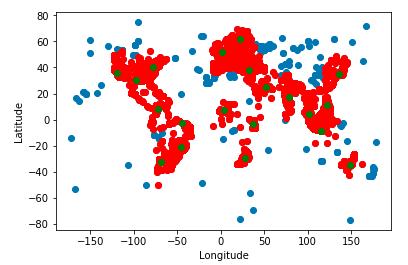
\includegraphics[scale=0.8]{Images/static}
\caption{k-Center Clustering using the static algorithm and $r=5.5$ on a subset of the twitter dataset. red : covered points, blue : uncovered points, green : centers points}
\label{fig:static}
\end{center}
\end{figure}

\section*{Questions 2,3 : Streaming Algorithm for k-Center Clustering}
\subsection*{Evaluate the Approximation Ratio}
\label{z_10}
\noindent
This second algorithm \cite{streaming} is also an algorithm for the k-center clustering problem. This time, it's a streaming algorithm which only stores $O(kz)$ points in memory and takes into account z outliers which will be ignored for the clustering. It achieves a (4+$\epsilon$)-approximation to the optimal clustering radius.\\
\subsubsection*{Results of the Streaming Algorithm}
\noindent
The results of the streaming algoritm when k=20, z=10 are not good at all (fig \ref{fig:sa_z_10}). The final radius is high and thus almost all the areas of the clusters overlap between eachother.
\begin{figure}[H]
\begin{center}
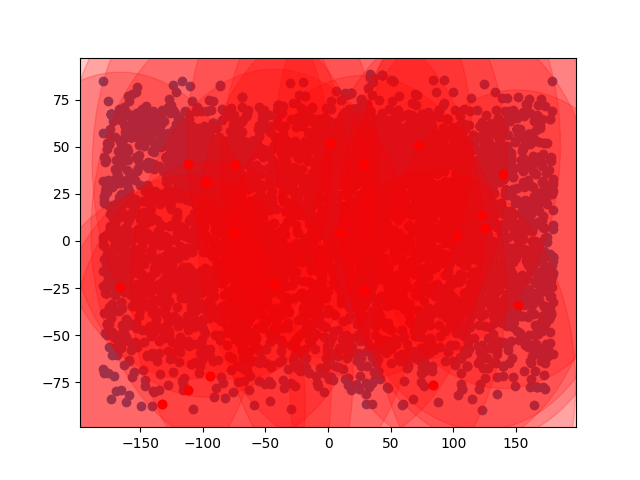
\includegraphics[scale=0.7]{Images/sa_z_10}
\caption{Result of the k-center clustering algorithm for k=20 and z=10. The algorithm finds 20 centers, each of them with a radius $r=114.04$.}
\label{fig:sa_z_10}
\end{center}
\end{figure}
\noindent
\textbf{In the instructions of the exercice, it's written : "To this end, you should try to give an upper bound on the optimum solution". And several lines below : "You should also discuss how you computed a lower bound on the optimum solution". I guess, the second one is the valid one but I did the first one before realizing it. In the following, I first propose a way to compute this upper bound and then the lower bound.}
\subsubsection*{Upper bound}
\noindent
A naïve approach would be to cover the range of the dataset by squares :
\begin{enumerate}
\item Compute the minimum and maximum of both axes (the dataset has only two columns) in order to get the enclosing rectangle
\item Find the minimum length $l$ to cover the enclosing rectangle by $k$ squares of length $l$
\item Fix a circle at the center of each square of radius $r'=\sqrt{2}\frac{l}{2}$
\end{enumerate}
This algorithm works because any square of length $l$ can be covered by a circle of radius $\sqrt{2}l$. In this case, we are able to cover the enclosing rectangle without taking care of the outliers with 18 squares of length 60 (fig \ref{fig:enclosing_with_squares}) and hence 18 circles of radius $r=\frac{60}{2}\sqrt{2}\simeq 42.42$ (fig \ref{fig:enclosing_with_circles}).\\
Allowing $z$ outliers will only reduces the radius of each circle. Then we found an upper bound (not tight at all) for the optimal solution : $r=42.42$.
\begin{figure}[H]
\centering
\begin{minipage}{.45\textwidth}
  \begin{center}
  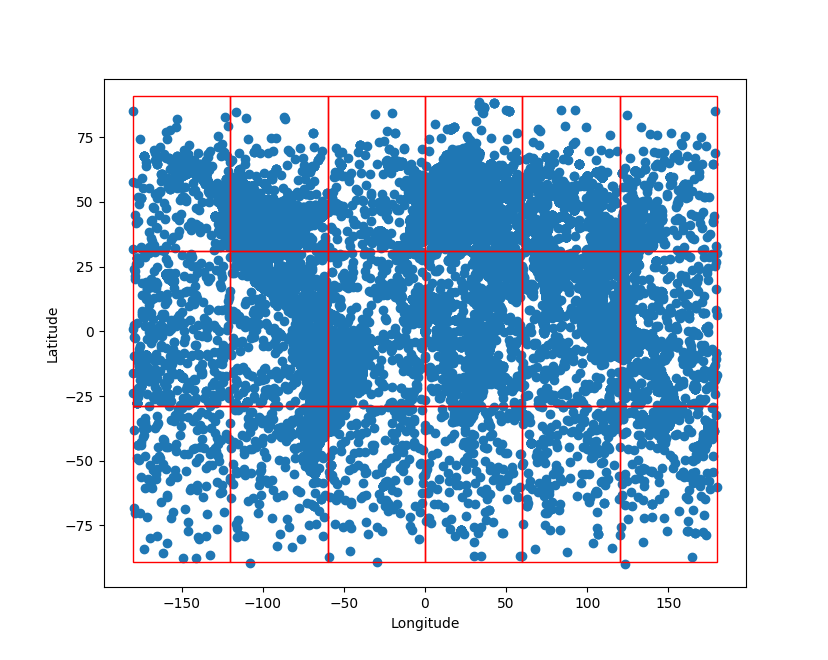
\includegraphics[scale=0.4]{Images/enclosing_with_squares}
  \caption{Covering the dataset with squares of length $l=60$ (it looks like rectangles because both axis don't have the same scale}
  \label{fig:enclosing_with_squares}
  \end{center}
\end{minipage}%
\hfill
\begin{minipage}{.45\textwidth}
  \begin{center}
  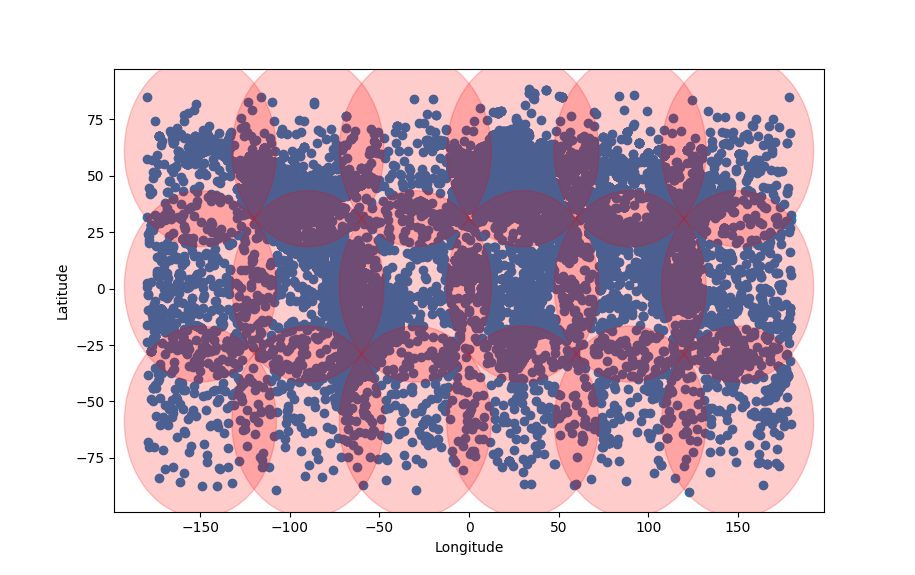
\includegraphics[scale=0.4]{Images/enclosing_with_circles}
  \caption{Covering the dataset using circles of radius $r'=30\sqrt{2}$}
  \label{fig:enclosing_with_circles}
  \end{center}
\end{minipage}
\end{figure}
\noindent
The approximation ratio is $A=\frac{\text{Radius Streaming Algorithm}}{\text{Radius from Upper Bound to the Optimal Solution}}=\frac{114.04}{42.42}=2.68$. This is actually a lower bound on the approximation ratio of the algorithm.

\subsubsection*{Lower Bound}
\noindent
A simple way to compute the lower bound for this problem is to compute a set of k+z+1 points which have the biggest distances between eachother. Indeed, if the minimum distance between k+z+1 points is $d$ then the algorithm won't be able to have a better solution because as most $z$ of these points will be outliers and the other ones will have to belong some cluster.\\
Thus a simple algorithm is :
\begin{enumerate}
\item Choose n points (the more the better), centers=$\emptyset$
\item Compute the distances between these points and add the 2 furthest points as centers
\item Compute the distances between the points and the centers
\item Add to the centers the point which is the furthest away from the centers
\item Go back to step 3 until k+z+1 points have been added to the centers
\end{enumerate}
\begin{figure}[H]
\begin{center}
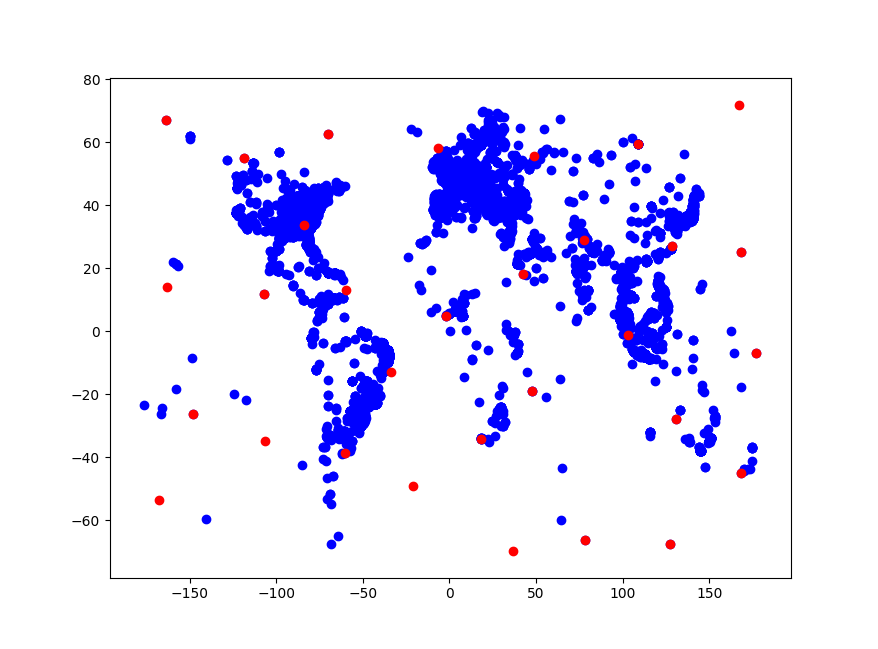
\includegraphics[scale=0.5]{Images/lower_bound}
\caption{k+z+1-centers with the above algorithm when k=20, z=10. Red:centers,blue:dataset. The minimum distance between all the centers is 33.65.}
\label{fig:lower_bound}
\end{center}
\end{figure}
In the first part, we found a clustering with a radius $r=114$. We know from fig \ref{fig:lower_bound} that the radius of an optimal solution can't be lower than 33.65. Then the approximation ratio is $\leq \frac{114}{33.65}=3.38$. Thus, the twitter data seems to not be far from the worst case scenario ($O(4+\epsilon)$).

\subsection*{Evaluate the Streaming Algorithm Depending on z}
\subsubsection*{Approximation Ratio}
\begin{figure}[H]
\begin{center}
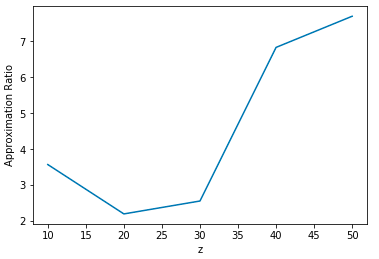
\includegraphics[scale=0.7]{Images/approx_ratio}
\caption{Evolution of the Approximation ratio depending on the value of z=\{10,20,30,40,50\}}
\label{fig:approx_ratio}
\end{center}
\end{figure}
\noindent
The shape of the approximation ratio (fig \ref{fig:approx_ratio}) is strange because allowing more outliers should reduces the value of the radius. Two hypothesis could explain this behaviour : 
\begin{enumerate}
\item The lower bound on the optimal radius decreases faster than the radius of the streaming algorithm
\item The streaming algorithm doesn't performs well when the batch size is too high
\end{enumerate}
It's actually a bit of those two hypothesis.\\
Indeed we can see of the fig \ref{fig:optimal_decreases} that the lower bound onto the optimal radius decreases quickly whereas the radius of the streaming algorithm doesn't have a special trend.\\
Moreover, the batch size is dependent on the number of outliers (because the batch size is $k+z$). At the begining of the algorithm, we compute the value of the inital radius $r$ as the mininmum distance of the first batch divides by 2. We observe on fig \ref{fig:fix_begining} that freezing the initial value of $r$ enables the streaming algorithm to decreases its radius when the number of allowed outliers increases (which is the natural behaviour).
\begin{figure}[H]
\centering
\begin{minipage}{.45\textwidth}
  \begin{center}
  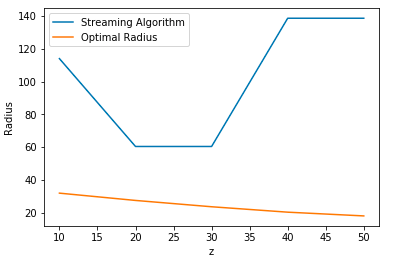
\includegraphics[scale=0.55]{Images/optimal_decreases}
  \caption{Evolution of the radius of the streaming algorithm and the lower bound of the optimal radius depending on the value of z=\{10,20,30,40,50\}}
  \label{fig:optimal_decreases}
  \end{center}
\end{minipage}%
\hfill
\begin{minipage}{.45\textwidth}
  \begin{center}
  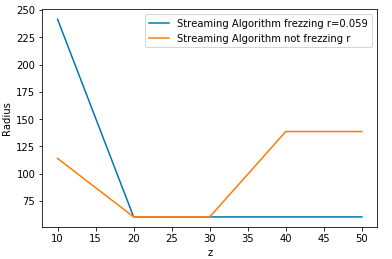
\includegraphics[scale=0.5]{Images/fix_begining}
  \caption{Evolution of the radius depending on the value of $z$ when freezing the initial value of the radius $r=0.059$ or when not freezing r}
  \label{fig:fix_begining}
  \end{center}
\end{minipage}
\end{figure}

\subsubsection{Time}
\noindent
The time spent by the algorithm is quite high because the algorithms are coded in Python (which is a slow language). Moreover we observe by comparing the fig \ref{fig:optimal_decreases} and fig \ref{fig:time}, that the time spend by the algorithm is negatively correlated with the value of the radius at the end of the algorithm.
\begin{figure}[H]
\begin{center}
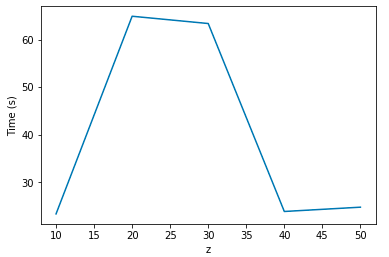
\includegraphics[scale=0.7]{Images/time}
\caption{Evolution of the time spent by the algorithm depending on the number of outliers z=\{10,20,30,40,50\}}
\label{fig:time}
\end{center}
\end{figure}

\section*{Conclusion}
\noindent
This report is a bit longer than expected but some things needed to be explained. The static algorithm in the first part performs quite well but is limited by the memory of the computer. On an another side, the streaming algorithm is memory efficient but we can't say that it performs well because tuning some parameters may change totally the value of the final radius (ex: the initial value of $r$). However, we can minimize these imperfections by reducing the value of $\alpha$, even if the time spent by the algorithm will be longer. Finally, I accidently computed an upper bound for the optimal radius and it appears to be not bad at all and easy to compute (its radius is 42.42 when the optimal one can't be lower than 33.65).

\begin{thebibliography}{999}

\bibitem{static}Moses Charikar, Samir Khuller, David M. Mount, and Giri Narasimhan,\emph{Algorithms for facility location problems with outliers}. 
\bibitem{streaming}Richard Matthew McCutchen and Samir Khuller,\emph{Streaming algorithms for k-center clustering with outliers and with anonymity}. 

\end{thebibliography}


\end{document}